\section{Yo}

We take the hamiltonian
\begin{equation}
    H = - \sum_{i,j} J_{ij} \sigma_i \sigma_j
\end{equation}

Below the critical temperature and with boundary conditions allowing the presence of an interface, we can approximate the Ising model by the Solid-on-Solid (SOS) model : there is a strong anisotropy in the system unabling spins to be in the other phase. Taking the interface along the x-axis, it translates as the presence of an interface $h(x)$ where each spin is defined as $\sigma(x,y) = \sign(h(x)-y)$.
No overlapping exists between both phases.


The $\sign$ function is defined as 
\begin{align*}
    \sign(x) &= \begin{cases} +1 \text{ if } x > 0 \\ -1 \text{ otherwise} \end{cases} \nn
        \sign(h - y)\sign(h' - y) &= \begin{cases} 1 \text{ if } y < \min(h,h') \\ 1 \text{ if } y > \max(h,h') \\ -1 \text{ otherwise} \end{cases}
\end{align*}

As we've defined the spins, 
\begin{align*}
    \sigma(x,y) = \sign(h(x)-y) \implies \begin{cases} \text{if } y < h(x), \sigma = +1 \nn \text{if } y > h(x), \sigma = -1 \end{cases}
\end{align*}

Thus, 
\begin{align*}
    \sum_{y=0}^L \sign(h-y)\sign(h'-y)  =& \sum_0^{\min(h,h')} 1 + \sum_{\min(h,h')}^{\max(h,h')} -1 + \sum_{\max(h,h')}^L 1 \nn
    =& \min(h,h') - \max(h,h') + \min(h,h') + L - \max(h,h') \nn
    =& L + 2(\min(h,h')-\max(h,h')) \nn
    =&  L - 2 |h-h'|
\end{align*}

Because $\max(a,b)-\min(a,b) = |a-b|$


\section{SOS Hamiltonian}

\begin{align*}
    H &= - J \sum_{i,j} \sigma_i \sigma_j  \nn
    &= -J \sum_{x,y} \sigma_{x,y} ( \sigma_{x+1,y}+\sigma_{x-1,y}+\sigma_{x,y+1}+\sigma_{x,y-1} ) \nn
    &= -J \sum_{x,y} \sign(h_x-y) ( \sign(h_{x+1}-y)+\sign(h_{x-1}-y)+\sign(h_{x}-y-1)+\sign(h_{x}-y+1) ) \nn
    &= -J \sum_x (L-2) |h_x-h_{x+1}|)+(L-2) |h_x-h_{x-1}|)+(L-1)+(L-1) \nn
    H &= 4 J L_X (2-L_Y) +4J \sum_x |h_x-h_{x+1}|
\end{align*}


\section{Hamiltonian with a crossover hamiltonian}

This computation is useful for the Casimir effect. 
\begin{figure}
    \centering
    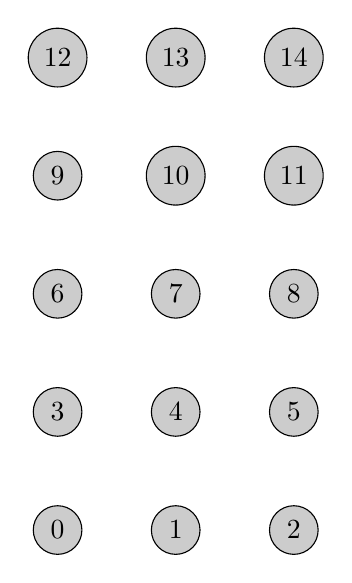
\begin{tikzpicture}[darkstyle/.style={circle,draw,fill=gray!40,minimum size=15}]
        \pgfmathsetmacro {\lx }{2}
        \pgfmathsetmacro {\ly }{4}
        \pgfmathtruncatemacro{\nnodes }{(1+\lx) * (1+\ly)}
        \pgfmathtruncatemacro{\nodes }{\nnodes-2}

        \foreach \x in {0,...,\lx}
        \foreach \y in {0,...,\ly}{
            \pgfmathtruncatemacro{\n}{\x + (1+\lx)*\y} 
            \node [darkstyle]  (\n) at (1.5*\x,1.5*\y) {\n};
        } 
        
%        \foreach \n in {0,...,\nodes}{
%            \pgfmathtruncatemacro{\m}{\n+1}
%            \draw (\n)--(\m);
%        }
    \end{tikzpicture}
    \caption{Finite size quantum well}
\end{figure}

We want to have a crossover at row $\alpha$. The system has a thickness $L_Y$ and we are removing a layer from it, to $L_Y-1$. For $\lambda=0$ the system is a normal system, while when we go to $\lambda=1$, we start decoupling the layer. The crossover hamiltonian hence gives
\begin{align*}
    H(\lambda) &= H_{SOS} - \sum_x (\lambda-1) J \sigma_\alpha (\sigma_{\alpha+1} + \sigma_{\alpha-1}) + (1-\lambda) J \sigma_{\alpha-1} \sigma_{\alpha+1} \nn
    &= H_{SOS} + (1-\lambda) J \sum_x \sigma_{\alpha-1} \sigma_{\alpha+1} - \sigma_\alpha (\sigma_{\alpha+1} + \sigma_{\alpha-1})
\end{align*}

(we remove a bond of energy J and add another one of energy $\lambda$ -> $\lambda-1$ for the decoupling layer, and vice-versa for the other layer)

Hence
$H(1) - H(0) = - J \sum_x \sigma_{\alpha-1} \sigma_{\alpha+1} - \sigma_\alpha (\sigma_{\alpha+1} + \sigma_{\alpha-1})$

\section{SOS Magnetization}

\begin{align*}
    m(y) &= \sum_{x,y} \sigma_{x,y} \nn
    &= \sum_{x,y} \sign(h_x-y) \nn
    &= \sum_{x,y} \sign(h_x-y) \sign(L_Y - y) \nn
    &= \sum_x 2 L_Y - 2 |L_Y - h_x|
\end{align*}

Le 2 LY est la car la somme se fait de -L a L, et non de 0 a L. Faudrait refaire les autres calculs en fait

\section{SOS Vertical Correlation Function}

\begin{align*}
    C_y(x,r) &= \frac{1}{L} \sum_y \sigma_{x,y} \sigma_{x,y+r} \nn
    &= \frac{1}{L} \sum_y \sign(h_x-y) \sign(h_x-y+r) \nn
    &= \frac{1}{L} \sum_y L-2 |h_x - h_x -r| \nn
    &= \frac{L - 2r}{L}
\end{align*}


\section{SOS Horizontal Correlation Function}

\begin{align*}
    C_x(r,y) &= \frac{1}{L_X} \sum_{x} \sigma_{x,y} \sigma_{x+r,y} \nn
    &= \frac{1}{L_X} \sum_x \sign( (h_x -y)(h_{x+r} -y))
\end{align*}

If we consider the interface beeing positioned at $y=0$ ,
\begin{align*}
    C_x(r,0) &= \frac{1}{L_X} \sum_x \sign(h_x h_{x+r})
\end{align*}

The fourrier transform of this function is thus
\begin{align*}
    \tilde{C}_x(q,0) &= \sum_{r=0}^{L-1} \frac{1}{L_X} \sum_x \sign(h_x h_{x+r}) e^{-2\pi i q \frac{r}{L}}
\end{align*}


\section{SOS Horizontal Bond Energy}
\begin{align*}
    E_x(y) &= - \frac{J}{L_X} \sum_x \sigma_{x,y} \sigma_{x+1,y} \nn
    &= -J C_x(1,y)
\end{align*}

\section{SOS Vertical Bond Energy}

\begin{align*}
    E_y(y) &= - \frac{J}{L_X} \sum_x \sigma_{x,y} \sigma_{x,y+1} \nn
    &= - \frac{J}{L_X} \sum_x \sign((h_x-y)(h_x -y-1)) \nn
\end{align*}

\begin{figure}[h]
  \begin{tabular}{|rl|l|l|}
  \hline
  \textbf{Variable} & & \textbf{Ising} & \textbf{Solid-On-Solid} 
  \rule[-2.5ex]{0pt}{7ex}\\ \hline
      Hamiltonian &$H$ & $- J \sum_{<ij>} \sigma_i \sigma_j - B \sum_i \sigma_i$ & $+4J \sum_x |h_x-h_{x+1}| - B \sum_x |h_x|$
  \rule[-2.5ex]{0pt}{7ex}\\ \hline
      Partition function &$Z$ & $\sum_{\sigma_i = \pm 1} e^{ \beta (J \sum_{<ij>} \sigma_i \sigma_j + B \sum_i \sigma_i )}$ & $\sum_{h_x} e^{-\beta ( 4J \sum_x |h_x-h_{x+1}| - B \sum_x |h_x|)}$
  \rule[-2.5ex]{0pt}{7ex}\\ \hline
      Magnetization &$m(y)$ &  $\sum_x \sigma_{x,y}$ & $\sum_x \sign(h_x-y)$
  \rule[-2.5ex]{0pt}{7ex}\\ \hline
      Vertical Correlation  &$C_y(x,r)$  & $\frac{1}{N} \sum_y \sigma_{x,y} \sigma_{x,y+r}$ & $\frac{N - 2r}{N}$
  \rule[-2.5ex]{0pt}{7ex}\\ \hline
      Horizontal Correlation  &$C_x(r,y)$ & $\frac{1}{L_X} \sum_{x} \sigma_{x,y} \sigma_{x+r,y}$ & $\frac{1}{L_X} \sum_x \sign( (h_x -y)(h_{x+r} -y))$
  \rule[-2.5ex]{0pt}{7ex}\\ \hline
  \end{tabular}
  \caption{Thermodynamic observables written in the Ising-model and their correspondence in the SOS model. The Hamiltonian and the Partition function are written with a steplike magnetic field $B(y) = B \sign(y)$}
  \label{ising-to-sos}
\end{figure}
